\documentclass[11pt]{article}
\usepackage[margin=0.75in]{geometry}
\usepackage[T1]{fontenc}
\usepackage[utf8]{inputenc}
\usepackage{lmodern}
\usepackage{microtype}
\usepackage{amsmath}
\usepackage{booktabs}
\usepackage{tabularx}
\usepackage{enumitem}
\usepackage{titlesec}
\usepackage{graphicx}
\usepackage{xcolor}
% Draft-only marker for sections still to rework; remove every \rework before submitting.
\newcommand{\rework}[1]{\noindent\colorbox{yellow!40}{\parbox{\dimexpr\linewidth-2\fboxsep}{%
  \small\textbf{REWORK:} #1}}\par}
\usepackage[hidelinks]{hyperref}

\setlist{nosep, leftmargin=*}
\titlespacing*{\section}{0pt}{1.0ex}{0.5ex}
\titlespacing*{\subsection}{0pt}{0.8ex}{0.3ex}
\titleformat*{\subsection}{\normalsize\bfseries}
\setlength{\parskip}{0.5ex}
\setlength{\parindent}{0pt}
\newcolumntype{Y}{>{\raggedright\arraybackslash}X}
\newcommand{\rhob}{\bar{\rho}}

\begin{document}

\begin{center}
  {\Large\bfseries Lab Report 2: An Agent that Diagnoses a Lattice-Stiffness GNN}\\[0.5ex]
  Jamie Carpenter (no team) \quad$\cdot$\quad AM/ME/CE 295 \quad$\cdot$\quad 1 November 2026\\
  \url{https://github.com/jamie-carpenter/lattice-gnn}
\end{center}

\section*{A \quad Project description \& goal}

\subsection*{A1 \quad Problem statement and goal}
Finite-element (FE) homogenization gives accurate effective stiffness for periodic strut lattices,
but it is too costly for screening catalogs of tens of thousands of unit cells. Therefore,
this project develops a graph neural network (GNN) as a surrogate model, trained on the 17,222
complete records of the Lumpe \& Stankovi\'c catalog~\cite{lumpe}. From the periodic graph of a
unit cell, the GNN predicts its three Young's and three shear moduli relative to the base-material
modulus $E_s$, together with three Poisson coupling terms. For the surrogate to be useful in
design, it must generalize to lattice families it has never seen before and return a physically
valid stiffness matrix (verified by checking the positive-definiteness of the matrix). The overall
goal of this project is to determine whether, \emph{at a fixed training budget, an LLM agent that
diagnoses why the GNN fails on held-out families reaches a lower held-out error than
hyperparameter optimization alone.} After each optimization round, the agent decides whether to
retune the hyperparameters, change the model structure or escalate the problem to me. If it only
ever chooses to retune, the optimizer alone will match its error at the same budget, and this
negative outcome would show that the agentic layer adds nothing over the non-agent baseline.

\subsection*{A2 \quad Related work}
\textbf{Domain.} Lumpe and Stankovi\'c~\cite{lumpe} built the catalog by decoding crystal networks
into periodic strut lattices and computed the effective stiffness of each lattice by FE
homogenization with Euler--Bernoulli beams ($E_s = 1$\,MPa, $\nu_s = 0.3$, $\rhob = 0.01$).
Indurkar et al.~\cite{indurkar} trained a message-passing GNN with periodic edges on 17,201
lattices from the same catalog [pp.~1, 3], but to classify lattices as stretching- or
bending-dominated, and reached 81.8\% validation accuracy on a random 90:10 split [p.~4]. Because a
random split places near-identical lattices on both sides, this project holds out whole families
instead. Grega et al.~\cite{grega} predicted the full stiffness tensor with an equivariant GNN
trained on 8,954 base lattices [p.~5]. Without constraints, their model predicted negative
eigenvalues for 30\% of lattices, and a positive-semi-definite output layer removed them [p.~7].
This result motivates both the positive-definiteness (PD) check and the PD output layer on the
structural menu. No published errors on this catalog are directly comparable to mine, so all
baselines in this project are my own.
\textbf{Agents.} Ferreira et al.~\cite{ferreira} found that, in a fixed search space and under the
same budget, classical optimizers (CMA-ES and the tree-structured Parzen estimator, TPE)
consistently outperformed LLM agents [p.~1], and that the best method
used the LLM only as an occasional informed perturbation [pp.~5, 8]. In a sequential setting, where
an agent reads the training logs and intervenes [p.~7], Huai et al.~\cite{huai} found the strongest
agent above conventional optimizers [p.~8], although agents still struggled with complex log
diagnosis [p.~1]. Osaro et al.~\cite{osaro} let agents edit the training code of an interatomic
potential and judged each change against a physically constrained scorecard [p.~1], which rejected
a change that lowered the error but broke an energy-drift limit [p.~3]; the PD check plays that
role here. Together, these studies suggest that an agent helps most when the decision draws on
information an optimizer does not see, and none of them applies such an agent to a GNN surrogate
for lattice stiffness.

\section*{B \quad Why an agent}

\subsection*{B1 \quad Why not a fixed script, an optimizer, or a single prompt}
The agent's goal is to make the surrogate reliable on unseen lattice families. It diagnoses why the
surrogate fails on those families and chooses the next step: (a) retune with new search ranges,
(b) change the model's structure with one option from a fixed menu, keeping earlier changes, or
(c) escalate to me, which is also how it proposes a structural change that is not on the menu. The
menu lists the changes the code supports, but the agent decides which failure each one should
address and when. Speeding up the search remains the job of the optimizer (Optuna), a tool that
both the agent and the baseline use (Fig.~\ref{fig:design}).
\textbf{Why not the optimizer alone.} Optuna adjusts numbers within a fixed structure and treats
the menu options as unordered categories. It therefore cannot read a failure pattern, such as
non-PD predictions in a few families that persist after retuning, and pick the option that targets
it. \textbf{Why not a fixed script.} If-then rules work when one symptom has one cause, but here the
same symptom can have several. A large error on one family may come from a poor learning-rate
range, a missing structural feature or corrupted labels, and telling these apart requires weighing
the per-family errors, the optimizer history and earlier decisions together.
\textbf{Why not a single prompt.} The decision depends on training runs that do not exist yet, so
the agent needs tools, memory across rounds and a stopping rule.

\section*{C \quad Agent design}

\subsection*{C1 \quad Agents, tools, data and information flow}
Figure~\ref{fig:design} shows the research loop, the baseline and the literature agent.
\begin{figure}[!tb]\centering
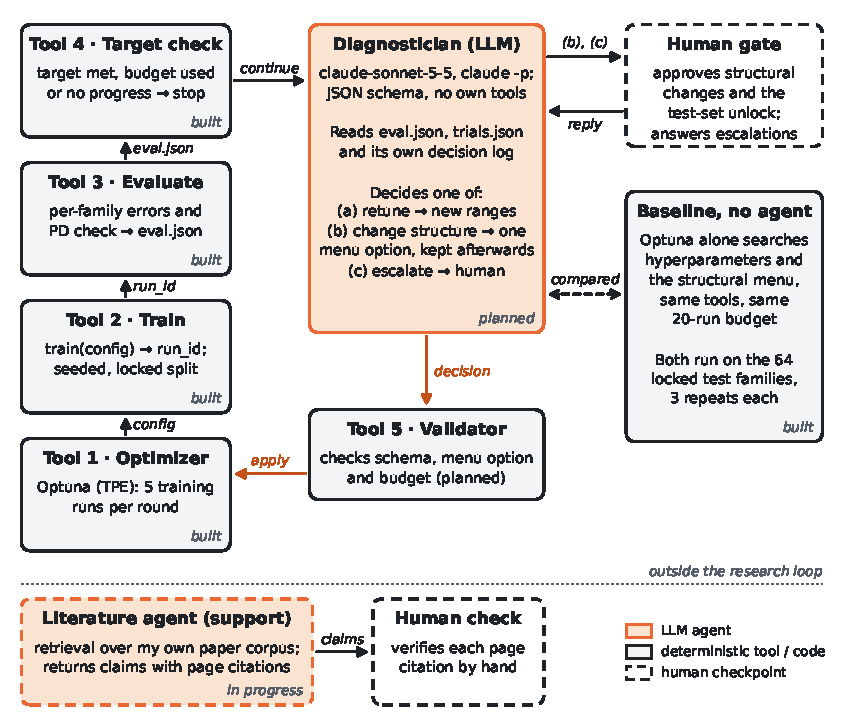
\includegraphics[width=0.78\linewidth]{figures/agent_design.pdf}
\caption{The research loop contains a single LLM decision. Each round, the optimizer launches five
training runs, the evaluation tool writes \texttt{eval.json} and code decides whether to stop;
otherwise the diagnostician's decision is validated and applied. I approve structural changes and
answer escalations. The baseline runs Optuna alone over the same hyperparameters and menu. Drawn
by a script written with Claude Code.}\label{fig:design}
\end{figure}

\subsection*{C2 \quad Why each part is needed: what breaks if it is removed}
\begin{itemize}
\item \textbf{Train (tool):} the agent has nothing to diagnose, and its choices have no effect.
\item \textbf{Evaluate (tool):} the agent cannot tell which families fail, and no LLM-free verdict
  remains.
\item \textbf{Optimizer (tool):} the agent would tune parameters itself, worse and at higher cost.
\item \textbf{Target check (code):} the agent could stop early or overspend.
\item \textbf{Validator (code):} off-menu or over-budget choices would run, giving the agent options
  the baseline lacks.
\item \textbf{Diagnostician (LLM):} the loop reduces to the optimizer alone, the ablation measured.
\item \textbf{Human gate:} structural changes and the test-set unlock go unreviewed.
\item \textbf{Literature agent:} the experiment runs, but I find and check related papers myself.
\end{itemize}

The diagnostician (\texttt{claude-sonnet-5-5} via \texttt{claude -p}) returns JSON and has no tools
of its own, so code runs every tool; it remembers earlier rounds only through its decision log.

\subsection*{C3 \quad Current working module}
The deterministic half of the loop and the optimizer baseline run end to end, covered by eleven
unit tests. The locked split groups the catalog into 456 families by crystal system and average
connectivity $Z$. Families with more than 200 lattices always go to training, and the rest are
split within each crystal system into 13,295, 2,039 and 1,928 lattices in 325, 67 and 64 families.
Of the 17,262 records split, the 17,222 with stiffness data are used (7 validation records lack it). Trained for 100 epochs on the full training split, the default model (four message-passing layers
of width 128) took about 1.5\,h on a laptop CPU (\texttt{runs/main-full}, Fig.~\ref{fig:runs}a).
Its validation loss, still falling at the end, reached 0.112 at epoch 97. On 2,032 validation lattices in 67 families, $R^2$ is 0.89--0.93 for the
moduli and 0.83--0.85 for the couplings, with median errors of 25--39\% and 0.041--0.048. However,
194 of these predictions (9.5\%) are not positive definite, whereas all 2,032 FE labels are (the
catalog's four non-PD labels all lie in the training set), so the violations come from the model
and are the failure the planned PD output layer targets. On a 2,000-lattice subset drawn from the
same split (\texttt{runs/main-2000}), the same model reached a validation loss of 0.223, median
modulus errors of 54--62\% and 7.9\% non-PD predictions on 239 of the validation lattices. About
eight times more data thus roughly halved the error, but it did not reduce the share of invalid
predictions; this is an observation, not a controlled scaling study.

One exploratory Optuna study on the subset (\texttt{runs/optuna-2000}), over six settings,
stopped after 13 of 20 runs (about 2\,h) because ten in a row brought no improvement (Fig.~\ref{fig:runs}b). Its best run reached a
validation loss of 0.224, no better than the untuned run, with 10\% non-PD predictions. Tuning alone therefore did not lower the held-out error on the subset,
which is where a diagnosis could add something, although a single study with one seed cannot
settle this.

\begin{figure}[!tb]\centering
\begin{minipage}[b]{0.50\linewidth}\centering
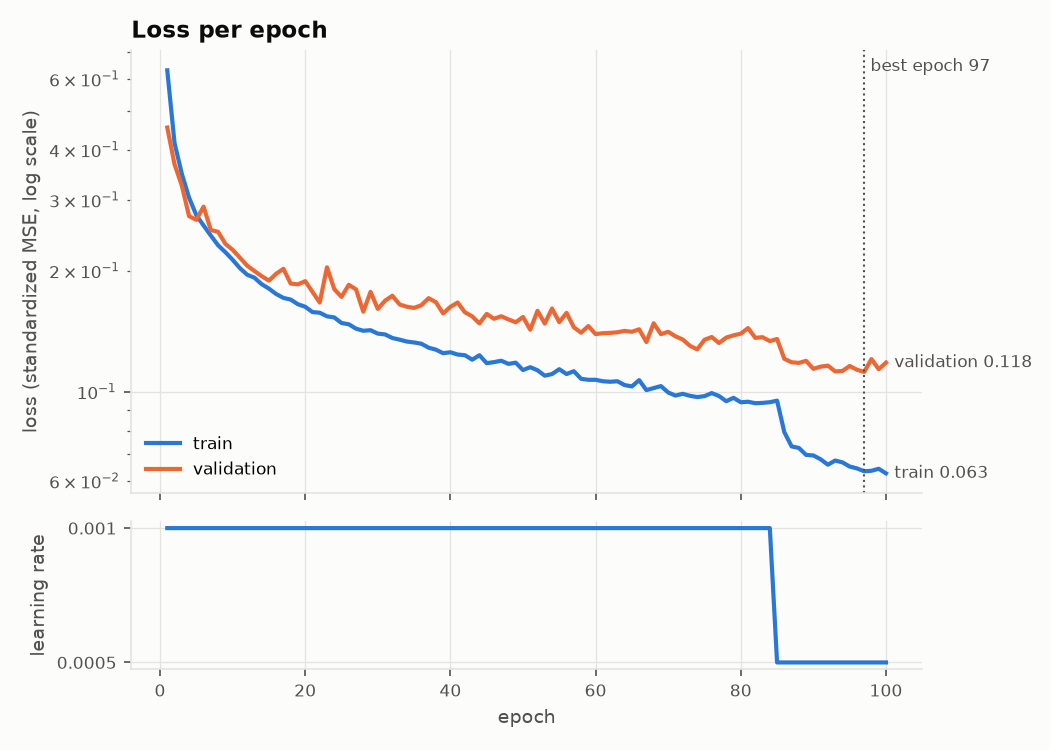
\includegraphics[height=4.0cm]{figures/mainfull_loss.png}\\[-0.5ex]{\small (a)}
\end{minipage}\hfill
\begin{minipage}[b]{0.48\linewidth}\centering
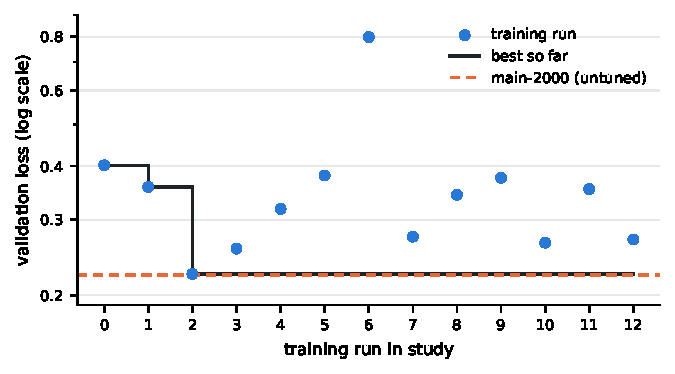
\includegraphics[height=3.8cm]{figures/optuna-2000_trials.pdf}\\[-0.5ex]{\small (b)}
\end{minipage}
\caption{(a) Loss (standardized MSE; 1.0 equals predicting the training mean) and learning rate
for \texttt{main-full}. (b) Validation loss of each run in the study \texttt{optuna-2000}, the best
so far, and the untuned \texttt{main-2000} run on the same data.}\label{fig:runs}
\end{figure}

\textbf{Module demo: the literature agent (Labs 4 and 5).} The literature agent lives in a separate
private repository, \texttt{capstone-agent}, which holds its instructions, memory, skills and
permissions. In Lab 4, I wrote its permissions as a specification
(\texttt{PERMISSIONS.md}) and enforced them through \texttt{.claude/settings.json}, which pins
\texttt{claude-opus-5-5}, allows only the course skills and pushes to \texttt{claude/} branches,
and denies merges, web tools, corpus edits and bypass mode. A weekday cloud routine that can reach
only \texttt{export.arxiv.org} writes an arXiv digest and opens a pull request that only I can
merge; on 29 October it found three new metamaterial papers. In Lab 5, I added retrieval over ten
papers on which this project rests, each pinned by edition, among them the catalog~\cite{lumpe} and
the PD output layers of Jekel et al.~\cite{jekel}. The index holds 376 chunks, each confined to one
page so that it carries its page number, and the agent may run only \texttt{retrieve.py} and
\texttt{check\_citations.py}, which confirms that every quote appears in the chunk it cites. In the
demo (\texttt{eval/transcript\_C.jsonl}), one \texttt{claude -p} call asked how Jekel et al. keep
the predicted stiffness positive definite. The agent passed the citation check for all three of
its quotes and answered that a Cholesky or
eigendecomposition output layer guarantees a PD output without adding learnable parameters
(\S6, p.~14), in 26\,s for US\$0.16. This is the source behind the \texttt{pd\_head} menu option.

On 25 questions written before any chunk existed, 19 of them answerable from the corpus, hit@5
(the share of answerable questions for which one of the five returned passages contains the
answer) was only 0.26--0.37 across embedding, hybrid and keyword search. The misses
share a cause: author names appear only in page headers and reference lists, so questions that name
a paper retrieve its bibliography, and paraphrases that span several papers match no single chunk.
The agent did, however, decline all six questions whose answer is not in the corpus, and I still
check each page citation by hand.

\section*{D \quad Evaluation}

\subsection*{D1 \quad LLM-free check and success}
\textbf{Physical validity.} Every predicted stiffness must be positive definite, so that any strain
stores positive energy. The couplings are the symmetric terms $c_{ij}=\nu_{ij}\sqrt{E_j/E_i}$ and the
moduli are positive, so the stiffness is positive definite exactly when the $3\times3$ block with
unit diagonal and $-c_{ij}$ off it is. Code checks that block's smallest eigenvalue against an
absolute tolerance of $3.6\times10^{-7}$, which is scale-free because the diagonal is one and bounds
the shift from rounding the couplings to single precision (derivation in \texttt{evaluate.py}).
\textbf{Success.} After exactly 20 training runs each, the agent's final model must have a lower
standardized MSE over the 64 locked test families (the optimizer's loss; median errors and the
non-PD rate are secondary) than the baseline's, by more than the spread across three repeats. Each
repeat's final model is its best validation run, and the test families are used once, at the end. I also report the non-PD rate and the runs
needed to reach the target defined below, and each escalation counts as not solved, so declining
cannot raise the score. To test the diagnosis itself, I plant three failures with known causes
(no PD output layer, a learning-rate range that excludes good values, and corrupted labels in one
family) and record whether the agent names the correct remedy.
\textbf{Thresholds.} The non-PD target is zero, because any non-PD prediction is physically
invalid. No specification fixes an acceptable error for the moduli, so I set no accuracy target by
eye. Instead, the target for counting runs is the best validation error the baseline reaches, and
every study uses its full budget. The catalog labels are rounded to three significant figures for
the moduli and three decimals for the couplings, which limits their resolution but is not a target.
\textbf{Checking each decision.} After each decision, code checks whether the next round lowered
the error of the targeted families and the non-PD rate, and whether a structural change had the
effect the agent predicted, and it logs both. Because the error also varies by chance, a drop
counts only if it exceeds the spread between runs with different seeds. Separately, Abaqus FE
simulations of selected lattices check the surrogate and the labels, not the decisions.
\textbf{Agent variability.} I pin the model ID and effort level, but \texttt{claude -p} cannot
set the temperature, so I seed training and Optuna and repeat each decision on the same frozen
reports about ten times.

\subsection*{D2 \quad Baseline}
The baseline is Optuna alone, with the same tools, 20-run budget, locked test families and three
repeats. It treats each menu option as an on/off setting, so it can try combinations of structural
changes from the start, whereas the agent adds one change per decision and keeps it. The baseline can reach every menu option the agent can, but the two
still search differently, so a gain may come from the stepwise, history-dependent search rather
than from the LLM's diagnosis. This is a limitation of the comparison; the planted failures test
the diagnosis directly. Results that depend on an off-menu change, which only the agent can
propose by escalating to me, are reported separately.

\section*{E \quad Plan and risks}

\subsection*{E1 \quad Milestones}
\textbf{By Lab Report 3 (Nov 15):} the \texttt{pd\_head} menu switch (PD by construction, with a
test); \texttt{validate.py} with a unit test per rule; the diagnostician making one validated
decision on the \texttt{main-full} report, with tokens and cost logged.
\textbf{By Lab Report 4 (Nov 29):} the loop with the human gate; \texttt{family\_balanced\_loss}
(then \texttt{physics\_residual}); agent and baseline studies on the full catalog, 3 repeats each
(about 180\,h at 1.5\,h per run), and the planted failures (about 90\,h); one evaluation on the
locked test families.

\subsection*{E2 \quad Biggest risk and question for the TAs}
Compute is the biggest risk: the studies and planted failures need about 270\,h of laptop CPU,
roughly 11 of the 14 days between Lab Reports 3 and 4, and even then 3 repeats per condition may
be too few to separate the agent from the baseline. \emph{Question:} is 3 repeats of a 20-run study enough for this
comparison, or should the budget be split differently?

\section*{Progress log}
\textbf{Done since Lab Report 1} (\texttt{LOG.md}, 29--31 Oct): the catalog's $Z_\text{avg}$
convention reproduced (257 of 17,262 records still differ); a family-grouping bug fixed; the
locked split frozen; the four loop tools built and tested; the first real training runs and Optuna
study; the success criteria fixed; Labs 4 and 5 built into the literature agent.
\textbf{Remaining:} the menu switches, the validator, the agent, the loop and the evaluation
harness; explaining the 257 $Z_\text{avg}$ mismatches and the 4 non-PD labels.
\textbf{Bottleneck:} CPU time for the full-catalog studies (E2). \textbf{Maintenance:} 27 commits
since 9 October and dated \texttt{LOG.md} entries for 18 and 29--31 October.

\section*{AI usage disclosure}
\textbf{Tools.} Claude Code (\texttt{claude-opus-5-5}, version 2.1.307) built this project under my
direction: it wrote the code, tests and figure scripts (25 of 27 commits carry its co-author line)
and drafted this report from \texttt{LOG.md} and my design worksheet. An earlier literature agent
(\texttt{claude-sonnet-5-5}) searched for related papers in two runs (\texttt{literature\_review/}).
For Labs 4 and 5, Claude Code drafted the permissions, the index change, the evaluation runs and
the notes in \texttt{capstone-agent}, and I approved each commit. \textbf{My role and checks.} I
made the design decisions, wrote the 25 retrieval questions, and reviewed each step and each
commit. Every number in this report comes from a logged run (\texttt{runs/} or
\texttt{capstone-agent/eval/}) or a cited paper. I read every cited paper and checked each cited page
against its PDF.

\begin{thebibliography}{9}\footnotesize\setlength{\itemsep}{0pt}
\bibitem{lumpe} T.~S. Lumpe, T.~Stankovi\'c. Exploring the property space of periodic cellular
  structures based on crystal networks. \emph{PNAS} 118(7), 2021. doi:10.1073/pnas.2003504118.
\bibitem{indurkar} P.~P. Indurkar, S.~Karlapati, A.~J.~D. Shaikeea, V.~S. Deshpande. Predicting
  deformation mechanisms in architected metamaterials using GNN. arXiv:2202.09427v2, 2022.
\bibitem{grega} I.~Grega, I.~Batatia, G.~Cs\'anyi, S.~Karlapati, V.~S. Deshpande.
  Energy-conserving equivariant GNN for elasticity of lattice architected metamaterials. ICLR 2024,
  arXiv:2401.16914v2.
\bibitem{ferreira} F.~Ferreira, L.~Wobbe, A.~Krishnakumar, F.~Hutter, A.~Zela. Can LLMs beat
  classical hyperparameter optimization algorithms? A study on autoresearch. arXiv:2603.24647v5,
  2026.
\bibitem{huai} T.~Huai, T.~Fan, X.~Chen, et al. AgentHPOBench: A benchmark for evaluating LLM
  agents as sequential hyperparameter optimizers. arXiv:2607.29626, 2026.
\bibitem{osaro} E.~Osaro, S.~Adhikari, S.~Zavitsanou, K.~Parker, D.~Rocca. MLIPilot: LLM-driven
  auto-research for machine-learned interatomic potentials. arXiv:2605.30889v1, 2026.
\bibitem{jekel} C.~F. Jekel, K.~E. Swartz, D.~A. White, D.~A. Tortorelli, S.~E. Watts. Neural
network layers for prediction of positive definite elastic stiffness tensors. arXiv:2203.13938v1,
2022.
\end{thebibliography}

\end{document}
